% Options for packages loaded elsewhere
% Options for packages loaded elsewhere
\PassOptionsToPackage{unicode}{hyperref}
\PassOptionsToPackage{hyphens}{url}
\PassOptionsToPackage{dvipsnames,svgnames,x11names}{xcolor}
%
\documentclass[
  letterpaper,
  DIV=11,
  numbers=noendperiod]{scrartcl}
\usepackage{xcolor}
\usepackage{amsmath,amssymb}
\setcounter{secnumdepth}{-\maxdimen} % remove section numbering
\usepackage{iftex}
\ifPDFTeX
  \usepackage[T1]{fontenc}
  \usepackage[utf8]{inputenc}
  \usepackage{textcomp} % provide euro and other symbols
\else % if luatex or xetex
  \usepackage{unicode-math} % this also loads fontspec
  \defaultfontfeatures{Scale=MatchLowercase}
  \defaultfontfeatures[\rmfamily]{Ligatures=TeX,Scale=1}
\fi
\usepackage{lmodern}
\ifPDFTeX\else
  % xetex/luatex font selection
\fi
% Use upquote if available, for straight quotes in verbatim environments
\IfFileExists{upquote.sty}{\usepackage{upquote}}{}
\IfFileExists{microtype.sty}{% use microtype if available
  \usepackage[]{microtype}
  \UseMicrotypeSet[protrusion]{basicmath} % disable protrusion for tt fonts
}{}
\makeatletter
\@ifundefined{KOMAClassName}{% if non-KOMA class
  \IfFileExists{parskip.sty}{%
    \usepackage{parskip}
  }{% else
    \setlength{\parindent}{0pt}
    \setlength{\parskip}{6pt plus 2pt minus 1pt}}
}{% if KOMA class
  \KOMAoptions{parskip=half}}
\makeatother
% Make \paragraph and \subparagraph free-standing
\makeatletter
\ifx\paragraph\undefined\else
  \let\oldparagraph\paragraph
  \renewcommand{\paragraph}{
    \@ifstar
      \xxxParagraphStar
      \xxxParagraphNoStar
  }
  \newcommand{\xxxParagraphStar}[1]{\oldparagraph*{#1}\mbox{}}
  \newcommand{\xxxParagraphNoStar}[1]{\oldparagraph{#1}\mbox{}}
\fi
\ifx\subparagraph\undefined\else
  \let\oldsubparagraph\subparagraph
  \renewcommand{\subparagraph}{
    \@ifstar
      \xxxSubParagraphStar
      \xxxSubParagraphNoStar
  }
  \newcommand{\xxxSubParagraphStar}[1]{\oldsubparagraph*{#1}\mbox{}}
  \newcommand{\xxxSubParagraphNoStar}[1]{\oldsubparagraph{#1}\mbox{}}
\fi
\makeatother

\usepackage{color}
\usepackage{fancyvrb}
\newcommand{\VerbBar}{|}
\newcommand{\VERB}{\Verb[commandchars=\\\{\}]}
\DefineVerbatimEnvironment{Highlighting}{Verbatim}{commandchars=\\\{\}}
% Add ',fontsize=\small' for more characters per line
\usepackage{framed}
\definecolor{shadecolor}{RGB}{241,243,245}
\newenvironment{Shaded}{\begin{snugshade}}{\end{snugshade}}
\newcommand{\AlertTok}[1]{\textcolor[rgb]{0.68,0.00,0.00}{#1}}
\newcommand{\AnnotationTok}[1]{\textcolor[rgb]{0.37,0.37,0.37}{#1}}
\newcommand{\AttributeTok}[1]{\textcolor[rgb]{0.40,0.45,0.13}{#1}}
\newcommand{\BaseNTok}[1]{\textcolor[rgb]{0.68,0.00,0.00}{#1}}
\newcommand{\BuiltInTok}[1]{\textcolor[rgb]{0.00,0.23,0.31}{#1}}
\newcommand{\CharTok}[1]{\textcolor[rgb]{0.13,0.47,0.30}{#1}}
\newcommand{\CommentTok}[1]{\textcolor[rgb]{0.37,0.37,0.37}{#1}}
\newcommand{\CommentVarTok}[1]{\textcolor[rgb]{0.37,0.37,0.37}{\textit{#1}}}
\newcommand{\ConstantTok}[1]{\textcolor[rgb]{0.56,0.35,0.01}{#1}}
\newcommand{\ControlFlowTok}[1]{\textcolor[rgb]{0.00,0.23,0.31}{\textbf{#1}}}
\newcommand{\DataTypeTok}[1]{\textcolor[rgb]{0.68,0.00,0.00}{#1}}
\newcommand{\DecValTok}[1]{\textcolor[rgb]{0.68,0.00,0.00}{#1}}
\newcommand{\DocumentationTok}[1]{\textcolor[rgb]{0.37,0.37,0.37}{\textit{#1}}}
\newcommand{\ErrorTok}[1]{\textcolor[rgb]{0.68,0.00,0.00}{#1}}
\newcommand{\ExtensionTok}[1]{\textcolor[rgb]{0.00,0.23,0.31}{#1}}
\newcommand{\FloatTok}[1]{\textcolor[rgb]{0.68,0.00,0.00}{#1}}
\newcommand{\FunctionTok}[1]{\textcolor[rgb]{0.28,0.35,0.67}{#1}}
\newcommand{\ImportTok}[1]{\textcolor[rgb]{0.00,0.46,0.62}{#1}}
\newcommand{\InformationTok}[1]{\textcolor[rgb]{0.37,0.37,0.37}{#1}}
\newcommand{\KeywordTok}[1]{\textcolor[rgb]{0.00,0.23,0.31}{\textbf{#1}}}
\newcommand{\NormalTok}[1]{\textcolor[rgb]{0.00,0.23,0.31}{#1}}
\newcommand{\OperatorTok}[1]{\textcolor[rgb]{0.37,0.37,0.37}{#1}}
\newcommand{\OtherTok}[1]{\textcolor[rgb]{0.00,0.23,0.31}{#1}}
\newcommand{\PreprocessorTok}[1]{\textcolor[rgb]{0.68,0.00,0.00}{#1}}
\newcommand{\RegionMarkerTok}[1]{\textcolor[rgb]{0.00,0.23,0.31}{#1}}
\newcommand{\SpecialCharTok}[1]{\textcolor[rgb]{0.37,0.37,0.37}{#1}}
\newcommand{\SpecialStringTok}[1]{\textcolor[rgb]{0.13,0.47,0.30}{#1}}
\newcommand{\StringTok}[1]{\textcolor[rgb]{0.13,0.47,0.30}{#1}}
\newcommand{\VariableTok}[1]{\textcolor[rgb]{0.07,0.07,0.07}{#1}}
\newcommand{\VerbatimStringTok}[1]{\textcolor[rgb]{0.13,0.47,0.30}{#1}}
\newcommand{\WarningTok}[1]{\textcolor[rgb]{0.37,0.37,0.37}{\textit{#1}}}

\usepackage{longtable,booktabs,array}
\usepackage{calc} % for calculating minipage widths
% Correct order of tables after \paragraph or \subparagraph
\usepackage{etoolbox}
\makeatletter
\patchcmd\longtable{\par}{\if@noskipsec\mbox{}\fi\par}{}{}
\makeatother
% Allow footnotes in longtable head/foot
\IfFileExists{footnotehyper.sty}{\usepackage{footnotehyper}}{\usepackage{footnote}}
\makesavenoteenv{longtable}
\usepackage{graphicx}
\makeatletter
\newsavebox\pandoc@box
\newcommand*\pandocbounded[1]{% scales image to fit in text height/width
  \sbox\pandoc@box{#1}%
  \Gscale@div\@tempa{\textheight}{\dimexpr\ht\pandoc@box+\dp\pandoc@box\relax}%
  \Gscale@div\@tempb{\linewidth}{\wd\pandoc@box}%
  \ifdim\@tempb\p@<\@tempa\p@\let\@tempa\@tempb\fi% select the smaller of both
  \ifdim\@tempa\p@<\p@\scalebox{\@tempa}{\usebox\pandoc@box}%
  \else\usebox{\pandoc@box}%
  \fi%
}
% Set default figure placement to htbp
\def\fps@figure{htbp}
\makeatother





\setlength{\emergencystretch}{3em} % prevent overfull lines

\providecommand{\tightlist}{%
  \setlength{\itemsep}{0pt}\setlength{\parskip}{0pt}}



 


\KOMAoption{captions}{tableheading}
\makeatletter
\@ifpackageloaded{tcolorbox}{}{\usepackage[skins,breakable]{tcolorbox}}
\@ifpackageloaded{fontawesome5}{}{\usepackage{fontawesome5}}
\definecolor{quarto-callout-color}{HTML}{909090}
\definecolor{quarto-callout-note-color}{HTML}{0758E5}
\definecolor{quarto-callout-important-color}{HTML}{CC1914}
\definecolor{quarto-callout-warning-color}{HTML}{EB9113}
\definecolor{quarto-callout-tip-color}{HTML}{00A047}
\definecolor{quarto-callout-caution-color}{HTML}{FC5300}
\definecolor{quarto-callout-color-frame}{HTML}{acacac}
\definecolor{quarto-callout-note-color-frame}{HTML}{4582ec}
\definecolor{quarto-callout-important-color-frame}{HTML}{d9534f}
\definecolor{quarto-callout-warning-color-frame}{HTML}{f0ad4e}
\definecolor{quarto-callout-tip-color-frame}{HTML}{02b875}
\definecolor{quarto-callout-caution-color-frame}{HTML}{fd7e14}
\makeatother
\makeatletter
\@ifpackageloaded{caption}{}{\usepackage{caption}}
\AtBeginDocument{%
\ifdefined\contentsname
  \renewcommand*\contentsname{Table of contents}
\else
  \newcommand\contentsname{Table of contents}
\fi
\ifdefined\listfigurename
  \renewcommand*\listfigurename{List of Figures}
\else
  \newcommand\listfigurename{List of Figures}
\fi
\ifdefined\listtablename
  \renewcommand*\listtablename{List of Tables}
\else
  \newcommand\listtablename{List of Tables}
\fi
\ifdefined\figurename
  \renewcommand*\figurename{Figure}
\else
  \newcommand\figurename{Figure}
\fi
\ifdefined\tablename
  \renewcommand*\tablename{Table}
\else
  \newcommand\tablename{Table}
\fi
}
\@ifpackageloaded{float}{}{\usepackage{float}}
\floatstyle{ruled}
\@ifundefined{c@chapter}{\newfloat{codelisting}{h}{lop}}{\newfloat{codelisting}{h}{lop}[chapter]}
\floatname{codelisting}{Listing}
\newcommand*\listoflistings{\listof{codelisting}{List of Listings}}
\makeatother
\makeatletter
\makeatother
\makeatletter
\@ifpackageloaded{caption}{}{\usepackage{caption}}
\@ifpackageloaded{subcaption}{}{\usepackage{subcaption}}
\makeatother
\usepackage{bookmark}
\IfFileExists{xurl.sty}{\usepackage{xurl}}{} % add URL line breaks if available
\urlstyle{same}
\hypersetup{
  pdftitle={Chapter 4: Computational Energy Analysis of Newton's Method},
  pdfauthor={Energy-Efficient Computing Research},
  colorlinks=true,
  linkcolor={blue},
  filecolor={Maroon},
  citecolor={Blue},
  urlcolor={Blue},
  pdfcreator={LaTeX via pandoc}}


\title{Chapter 4: Computational Energy Analysis of Newton's Method}
\usepackage{etoolbox}
\makeatletter
\providecommand{\subtitle}[1]{% add subtitle to \maketitle
  \apptocmd{\@title}{\par {\large #1 \par}}{}{}
}
\makeatother
\subtitle{A Study of the General nth Root Algorithm}
\author{Energy-Efficient Computing Research}
\date{}
\begin{document}
\maketitle


\subsection{Introduction}\label{introduction}

\begin{tcolorbox}[enhanced jigsaw, rightrule=.15mm, colbacktitle=quarto-callout-note-color!10!white, titlerule=0mm, toptitle=1mm, colframe=quarto-callout-note-color-frame, bottomtitle=1mm, coltitle=black, arc=.35mm, breakable, title=\textcolor{quarto-callout-note-color}{\faInfo}\hspace{0.5em}{Research Question}, bottomrule=.15mm, toprule=.15mm, colback=white, left=2mm, opacityback=0, opacitybacktitle=0.6, leftrule=.75mm]

How much \textbf{computational energy} does Newton's method consume when
generalized to find any nth root?

\end{tcolorbox}

\begin{itemize}
\tightlist
\item
  Newton's method is a powerful algorithm for finding roots
\item
  We've generalized it from square roots to {\textbf{any nth root}}
\item
  Why does energy matter?

  \begin{itemize}
  \tightlist
  \item
    🔋 Battery life in mobile devices
  \item
    🌱 Server costs and carbon footprint
  \item
    ⚡ Real-time system constraints
  \item
    📱 IoT and edge computing limitations
  \end{itemize}
\end{itemize}

\subsection{The General Algorithm}\label{the-general-algorithm}

\begin{Shaded}
\begin{Highlighting}[]
\KeywordTok{def}\NormalTok{ newtons\_nth\_root(n: }\BuiltInTok{int}\NormalTok{, value: }\BuiltInTok{float}\NormalTok{, guess: }\BuiltInTok{float} \OperatorTok{=} \FloatTok{1.0}\NormalTok{):}
    \CommentTok{"""Find the nth root of a value using Newton\textquotesingle{}s method"""}
\NormalTok{    tolerance }\OperatorTok{=} \FloatTok{0.0001}
    
    \ControlFlowTok{while} \BuiltInTok{abs}\NormalTok{(guess}\OperatorTok{**}\NormalTok{n }\OperatorTok{{-}}\NormalTok{ value) }\OperatorTok{\textgreater{}}\NormalTok{ tolerance:}
        \CommentTok{\# Newton\textquotesingle{}s formula: y\_new = y {-} f(y)/f\textquotesingle{}(y)}
        \CommentTok{\# For f(y) = y\^{}n {-} value:}
\NormalTok{        guess\_new }\OperatorTok{=}\NormalTok{ guess }\OperatorTok{{-}}\NormalTok{ (guess}\OperatorTok{**}\NormalTok{n }\OperatorTok{{-}}\NormalTok{ value) }\OperatorTok{/}\NormalTok{ (n }\OperatorTok{*}\NormalTok{ guess}\OperatorTok{**}\NormalTok{(n}\OperatorTok{{-}}\DecValTok{1}\NormalTok{))}
\NormalTok{        guess }\OperatorTok{=}\NormalTok{ guess\_new}
    
    \ControlFlowTok{return}\NormalTok{ guess}
\end{Highlighting}
\end{Shaded}

~

\begin{tcolorbox}[enhanced jigsaw, rightrule=.15mm, colbacktitle=quarto-callout-tip-color!10!white, titlerule=0mm, toptitle=1mm, colframe=quarto-callout-tip-color-frame, bottomtitle=1mm, coltitle=black, arc=.35mm, breakable, title=\textcolor{quarto-callout-tip-color}{\faLightbulb}\hspace{0.5em}{Mathematical Foundation}, bottomrule=.15mm, toprule=.15mm, colback=white, left=2mm, opacityback=0, opacitybacktitle=0.6, leftrule=.75mm]

\textbf{Quadratic convergence} means errors roughly {square each
iteration}!

This exponential error reduction is the key to Newton's energy
efficiency.

\end{tcolorbox}

\subsection{Energy Measurement Setup}\label{energy-measurement-setup}

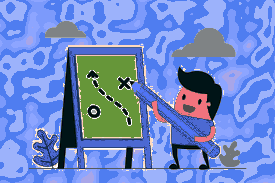
\includegraphics[width=0.45\linewidth,height=\textheight,keepaspectratio]{graphics/strategy_i.png}

\textbf{Energy Tracking Strategy}

\begin{itemize}
\tightlist
\item
  Count arithmetic operations per iteration
\item
  Measure wall-clock computation time\\
\item
  Track convergence behavior
\item
  Compare across different root degrees
\end{itemize}

\begin{center}\rule{0.5\linewidth}{0.5pt}\end{center}

\begin{Shaded}
\begin{Highlighting}[]
\ImportTok{import}\NormalTok{ time}

\KeywordTok{def}\NormalTok{ newtons\_nth\_root\_instrumented(n, value, guess}\OperatorTok{=}\FloatTok{1.0}\NormalTok{):}
\NormalTok{    iterations }\OperatorTok{=} \DecValTok{0}
\NormalTok{    operations\_count }\OperatorTok{=} \DecValTok{0}
\NormalTok{    start\_time }\OperatorTok{=}\NormalTok{ time.time()}
\NormalTok{    tolerance }\OperatorTok{=} \FloatTok{0.0001}
    \ControlFlowTok{while} \BuiltInTok{abs}\NormalTok{(guess}\OperatorTok{**}\NormalTok{n }\OperatorTok{{-}}\NormalTok{ value) }\OperatorTok{\textgreater{}}\NormalTok{ tolerance:}
\NormalTok{        iterations }\OperatorTok{+=} \DecValTok{1}
        
        \CommentTok{\# Count operations per iteration:}
        \CommentTok{\# {-} guess**n: (n{-}1) multiplications}
        \CommentTok{\# {-} guess**(n{-}1): (n{-}2) multiplications}
        \CommentTok{\# {-} Basic arithmetic: 3 operations}
\NormalTok{        operations\_count }\OperatorTok{+=}\NormalTok{ (n}\OperatorTok{{-}}\DecValTok{1}\NormalTok{) }\OperatorTok{+}\NormalTok{ (n}\OperatorTok{{-}}\DecValTok{2}\NormalTok{) }\OperatorTok{+} \DecValTok{3} \OperatorTok{+} \DecValTok{2}
        
\NormalTok{        guess }\OperatorTok{=}\NormalTok{ guess }\OperatorTok{{-}}\NormalTok{ (guess}\OperatorTok{**}\NormalTok{n }\OperatorTok{{-}}\NormalTok{ value) }\OperatorTok{/}\NormalTok{ (n }\OperatorTok{*}\NormalTok{ guess}\OperatorTok{**}\NormalTok{(n}\OperatorTok{{-}}\DecValTok{1}\NormalTok{))}
    
\NormalTok{    computation\_time }\OperatorTok{=}\NormalTok{ time.time() }\OperatorTok{{-}}\NormalTok{ start\_time}
    \ControlFlowTok{return}\NormalTok{ guess, iterations, computation\_time, operations\_count}

\CommentTok{\# print the results}
\NormalTok{results }\OperatorTok{=}\NormalTok{ newtons\_nth\_root\_instrumented(}\DecValTok{2}\NormalTok{,}\DecValTok{144}\NormalTok{)}
\BuiltInTok{print}\NormalTok{(}\SpecialStringTok{f"guess : }\SpecialCharTok{\{}\NormalTok{results[}\DecValTok{0}\NormalTok{]}\SpecialCharTok{\}}\SpecialStringTok{"}\NormalTok{)}
\BuiltInTok{print}\NormalTok{(}\SpecialStringTok{f"iterations : }\SpecialCharTok{\{}\NormalTok{results[}\DecValTok{1}\NormalTok{]}\SpecialCharTok{\}}\SpecialStringTok{"}\NormalTok{)}
\BuiltInTok{print}\NormalTok{(}\SpecialStringTok{f"comp\_time : }\SpecialCharTok{\{}\NormalTok{results[}\DecValTok{2}\NormalTok{]}\SpecialCharTok{\}}\SpecialStringTok{"}\NormalTok{)}
\BuiltInTok{print}\NormalTok{(}\SpecialStringTok{f"operations : }\SpecialCharTok{\{}\NormalTok{results[}\DecValTok{3}\NormalTok{]}\SpecialCharTok{\}}\SpecialStringTok{"}\NormalTok{)}
\end{Highlighting}
\end{Shaded}

\begin{center}\rule{0.5\linewidth}{0.5pt}\end{center}

\subsubsection{Results}\label{results}

\begin{Shaded}
\begin{Highlighting}[]
\NormalTok{results }\OperatorTok{=}\NormalTok{ newtons\_nth\_root\_instrumented(}\DecValTok{3}\NormalTok{,}\DecValTok{27}\NormalTok{)}
\BuiltInTok{print}\NormalTok{(}\SpecialStringTok{f"guess : }\SpecialCharTok{\{}\NormalTok{results[}\DecValTok{0}\NormalTok{]}\SpecialCharTok{\}}\SpecialStringTok{"}\NormalTok{)}
\BuiltInTok{print}\NormalTok{(}\SpecialStringTok{f"iterations : }\SpecialCharTok{\{}\NormalTok{results[}\DecValTok{1}\NormalTok{]}\SpecialCharTok{\}}\SpecialStringTok{"}\NormalTok{)}
\BuiltInTok{print}\NormalTok{(}\SpecialStringTok{f"comp\_time : }\SpecialCharTok{\{}\NormalTok{results[}\DecValTok{2}\NormalTok{]}\SpecialCharTok{\}}\SpecialStringTok{"}\NormalTok{)}
\BuiltInTok{print}\NormalTok{(}\SpecialStringTok{f"operations : }\SpecialCharTok{\{}\NormalTok{results[}\DecValTok{3}\NormalTok{]}\SpecialCharTok{\}}\SpecialStringTok{"}\NormalTok{)}
\end{Highlighting}
\end{Shaded}

\begin{verbatim}
guess : 3.0000005410641766
iterations : 7
comp_time : 1.0013580322265625e-05
operations : 56
\end{verbatim}

\begin{Shaded}
\begin{Highlighting}[]
\NormalTok{results }\OperatorTok{=}\NormalTok{ newtons\_nth\_root\_instrumented(}\DecValTok{3}\NormalTok{,}\DecValTok{27}\NormalTok{)}
\BuiltInTok{print}\NormalTok{(}\SpecialStringTok{f"guess : }\SpecialCharTok{\{}\NormalTok{results[}\DecValTok{0}\NormalTok{]}\SpecialCharTok{\}}\SpecialStringTok{"}\NormalTok{)}
\BuiltInTok{print}\NormalTok{(}\SpecialStringTok{f"iterations : }\SpecialCharTok{\{}\NormalTok{results[}\DecValTok{1}\NormalTok{]}\SpecialCharTok{\}}\SpecialStringTok{"}\NormalTok{)}
\BuiltInTok{print}\NormalTok{(}\SpecialStringTok{f"comp\_time : }\SpecialCharTok{\{}\NormalTok{results[}\DecValTok{2}\NormalTok{]}\SpecialCharTok{\}}\SpecialStringTok{"}\NormalTok{)}
\BuiltInTok{print}\NormalTok{(}\SpecialStringTok{f"operations : }\SpecialCharTok{\{}\NormalTok{results[}\DecValTok{3}\NormalTok{]}\SpecialCharTok{\}}\SpecialStringTok{"}\NormalTok{)}
\end{Highlighting}
\end{Shaded}

\begin{verbatim}
guess : 3.0000005410641766
iterations : 7
comp_time : 8.821487426757812e-06
operations : 56
\end{verbatim}

\begin{center}\rule{0.5\linewidth}{0.5pt}\end{center}

\subsection{Live Demo: Energy Analysis}\label{live-demo-energy-analysis}

\begin{Shaded}
\begin{Highlighting}[]
\ImportTok{import}\NormalTok{ time}

\KeywordTok{def}\NormalTok{ newtons\_nth\_root(n: }\BuiltInTok{int}\NormalTok{, value: }\BuiltInTok{float}\NormalTok{, guess: }\BuiltInTok{float} \OperatorTok{=} \FloatTok{1.0}\NormalTok{, verbose: }\BuiltInTok{bool} \OperatorTok{=} \VariableTok{True}\NormalTok{) }\OperatorTok{{-}\textgreater{}} \BuiltInTok{tuple}\NormalTok{:}
    \CommentTok{"""Find the nth root of a value using Newton\textquotesingle{}s method with performance analysis."""}
    \ControlFlowTok{if}\NormalTok{ n }\OperatorTok{\textless{}=} \DecValTok{0}\NormalTok{:}
        \ControlFlowTok{raise} \PreprocessorTok{ValueError}\NormalTok{(}\StringTok{"n must be a positive integer"}\NormalTok{)}
    \ControlFlowTok{if}\NormalTok{ value }\OperatorTok{\textless{}} \DecValTok{0} \KeywordTok{and}\NormalTok{ n }\OperatorTok{\%} \DecValTok{2} \OperatorTok{==} \DecValTok{0}\NormalTok{:}
        \ControlFlowTok{raise} \PreprocessorTok{ValueError}\NormalTok{(}\StringTok{"Cannot find even root of negative number"}\NormalTok{)}
    
\NormalTok{    tolerance }\OperatorTok{=} \FloatTok{0.0001}
\NormalTok{    iterations }\OperatorTok{=} \DecValTok{0}
\NormalTok{    operations\_count }\OperatorTok{=} \DecValTok{0}
\NormalTok{    start\_time }\OperatorTok{=}\NormalTok{ time.time()}
    
    \ControlFlowTok{while} \BuiltInTok{abs}\NormalTok{(guess}\OperatorTok{**}\NormalTok{n }\OperatorTok{{-}}\NormalTok{ value) }\OperatorTok{\textgreater{}}\NormalTok{ tolerance:}
\NormalTok{        iterations }\OperatorTok{+=} \DecValTok{1}
        
        \ControlFlowTok{if}\NormalTok{ verbose:}
            \BuiltInTok{print}\NormalTok{(}\SpecialStringTok{f"Iter }\SpecialCharTok{\{}\NormalTok{iterations}\SpecialCharTok{\}}\SpecialStringTok{: guess = }\SpecialCharTok{\{}\NormalTok{guess}\SpecialCharTok{:.4f\}}\SpecialStringTok{, error = }\SpecialCharTok{\{}\BuiltInTok{abs}\NormalTok{(guess}\OperatorTok{**}\NormalTok{n }\OperatorTok{{-}}\NormalTok{ value)}\SpecialCharTok{:.6f\}}\SpecialStringTok{"}\NormalTok{)}
        
\NormalTok{        operations\_this\_iteration }\OperatorTok{=}\NormalTok{ (n}\OperatorTok{{-}}\DecValTok{1}\NormalTok{) }\OperatorTok{+}\NormalTok{ (n}\OperatorTok{{-}}\DecValTok{2}\NormalTok{) }\OperatorTok{+} \DecValTok{3} \OperatorTok{+} \DecValTok{2}
\NormalTok{        operations\_count }\OperatorTok{+=}\NormalTok{ operations\_this\_iteration}
        
\NormalTok{        guess\_new }\OperatorTok{=}\NormalTok{ guess }\OperatorTok{{-}}\NormalTok{ (guess}\OperatorTok{**}\NormalTok{n }\OperatorTok{{-}}\NormalTok{ value) }\OperatorTok{/}\NormalTok{ (n }\OperatorTok{*}\NormalTok{ guess}\OperatorTok{**}\NormalTok{(n}\OperatorTok{{-}}\DecValTok{1}\NormalTok{))}
\NormalTok{        guess }\OperatorTok{=}\NormalTok{ guess\_new}
    
\NormalTok{    computation\_time }\OperatorTok{=}\NormalTok{ time.time() }\OperatorTok{{-}}\NormalTok{ start\_time}
    
    \ControlFlowTok{if}\NormalTok{ verbose:}
        \BuiltInTok{print}\NormalTok{(}\SpecialStringTok{f"✓ Converged in }\SpecialCharTok{\{}\NormalTok{iterations}\SpecialCharTok{\}}\SpecialStringTok{ iterations"}\NormalTok{)}
        \BuiltInTok{print}\NormalTok{(}\SpecialStringTok{f"✓ Total operations: }\SpecialCharTok{\{}\NormalTok{operations\_count}\SpecialCharTok{\}}\SpecialStringTok{"}\NormalTok{)}
        \BuiltInTok{print}\NormalTok{(}\SpecialStringTok{f"✓ Time: }\SpecialCharTok{\{}\NormalTok{computation\_time}\SpecialCharTok{:.6f\}}\SpecialStringTok{ seconds"}\NormalTok{)}
    
    \ControlFlowTok{return}\NormalTok{ guess, iterations, computation\_time, operations\_count}
\end{Highlighting}
\end{Shaded}

\begin{center}\rule{0.5\linewidth}{0.5pt}\end{center}

\subsection{Results: Energy Analysis}\label{results-energy-analysis}

\begin{tcolorbox}[enhanced jigsaw, rightrule=.15mm, colbacktitle=quarto-callout-note-color!10!white, titlerule=0mm, toptitle=1mm, colframe=quarto-callout-note-color-frame, bottomtitle=1mm, coltitle=black, arc=.35mm, breakable, title=\textcolor{quarto-callout-note-color}{\faInfo}\hspace{0.5em}{Live Demonstration}, bottomrule=.15mm, toprule=.15mm, colback=white, left=2mm, opacityback=0, opacitybacktitle=0.6, leftrule=.75mm]

Watch Newton's method converge in real-time with energy tracking!

\end{tcolorbox}

\begin{Shaded}
\begin{Highlighting}[]
\CommentTok{\# Quick demo: Square root of 16}
\NormalTok{result, iters, time\_taken, ops }\OperatorTok{=}\NormalTok{ newtons\_nth\_root(}\DecValTok{2}\NormalTok{, }\DecValTok{16}\NormalTok{, verbose}\OperatorTok{=}\VariableTok{True}\NormalTok{)}
\BuiltInTok{print}\NormalTok{(}\SpecialStringTok{f"Result: }\SpecialCharTok{\{}\NormalTok{result}\SpecialCharTok{:.6f\}}\SpecialStringTok{"}\NormalTok{)}
\end{Highlighting}
\end{Shaded}

\begin{Shaded}
\begin{Highlighting}[]
\CommentTok{\# Quick demo: Square root of 16}
\NormalTok{result, iters, time\_taken, ops }\OperatorTok{=}\NormalTok{ newtons\_nth\_root(}\DecValTok{2}\NormalTok{, }\DecValTok{16}\NormalTok{, verbose}\OperatorTok{=}\VariableTok{True}\NormalTok{)}
\BuiltInTok{print}\NormalTok{(}\SpecialStringTok{f"Result: }\SpecialCharTok{\{}\NormalTok{result}\SpecialCharTok{:.6f\}}\SpecialStringTok{"}\NormalTok{)}
\end{Highlighting}
\end{Shaded}

\begin{verbatim}
Iter 1: guess = 1.0000, error = 15.000000
Iter 2: guess = 8.5000, error = 56.250000
Iter 3: guess = 5.1912, error = 10.948313
Iter 4: guess = 4.1367, error = 1.111995
Iter 5: guess = 4.0023, error = 0.018065
✓ Converged in 5 iterations
✓ Total operations: 30
✓ Time: 0.000113 seconds
Result: 4.000001
\end{verbatim}

\begin{tcolorbox}[enhanced jigsaw, rightrule=.15mm, colbacktitle=quarto-callout-tip-color!10!white, titlerule=0mm, toptitle=1mm, colframe=quarto-callout-tip-color-frame, bottomtitle=1mm, coltitle=black, arc=.35mm, breakable, title=\textcolor{quarto-callout-tip-color}{\faLightbulb}\hspace{0.5em}{Key Observation}, bottomrule=.15mm, toprule=.15mm, colback=white, left=2mm, opacityback=0, opacitybacktitle=0.6, leftrule=.75mm]

Notice how quickly it converges - only {\textbf{2-3 iterations}} for
most calculations!

\end{tcolorbox}

\begin{center}\rule{0.5\linewidth}{0.5pt}\end{center}

\subsubsection{Energy Comp Across Root
Degrees}\label{energy-comp-across-root-degrees}

\begin{Shaded}
\begin{Highlighting}[]
\ImportTok{import}\NormalTok{ plotly.graph\_objects }\ImportTok{as}\NormalTok{ go}
\ImportTok{import}\NormalTok{ plotly.express }\ImportTok{as}\NormalTok{ px}
\ImportTok{from}\NormalTok{ plotly.subplots }\ImportTok{import}\NormalTok{ make\_subplots}
\ImportTok{import}\NormalTok{ pandas }\ImportTok{as}\NormalTok{ pd}

\CommentTok{\# Test cases for energy comparison}
\NormalTok{test\_cases }\OperatorTok{=}\NormalTok{ [}
\NormalTok{    (}\DecValTok{2}\NormalTok{, }\DecValTok{16}\NormalTok{, }\StringTok{"Square root of 16"}\NormalTok{), (}\DecValTok{3}\NormalTok{, }\DecValTok{27}\NormalTok{, }\StringTok{"Cube root of 27"}\NormalTok{),}
\NormalTok{    (}\DecValTok{4}\NormalTok{, }\DecValTok{81}\NormalTok{, }\StringTok{"Fourth root of 81"}\NormalTok{), (}\DecValTok{5}\NormalTok{, }\DecValTok{32}\NormalTok{, }\StringTok{"Fifth root of 32"}\NormalTok{),}
\NormalTok{    (}\DecValTok{6}\NormalTok{, }\DecValTok{64}\NormalTok{, }\StringTok{"Sixth root of 64"}\NormalTok{), (}\DecValTok{8}\NormalTok{, }\DecValTok{256}\NormalTok{, }\StringTok{"Eighth root of 256"}\NormalTok{),}
\NormalTok{    (}\DecValTok{10}\NormalTok{, }\DecValTok{1024}\NormalTok{, }\StringTok{"Tenth root of 1024"}\NormalTok{),}
\NormalTok{]}

\CommentTok{\# Collect data for plotting}
\NormalTok{data }\OperatorTok{=}\NormalTok{ []}
\ControlFlowTok{for}\NormalTok{ n, value, description }\KeywordTok{in}\NormalTok{ test\_cases:}
\NormalTok{    result, iterations, time\_taken, operations }\OperatorTok{=}\NormalTok{ newtons\_nth\_root(n, value, verbose}\OperatorTok{=}\VariableTok{False}\NormalTok{)}
\NormalTok{    ops\_per\_iter }\OperatorTok{=}\NormalTok{ operations }\OperatorTok{/}\NormalTok{ iterations}
\NormalTok{    data.append(\{}
        \StringTok{\textquotesingle{}root\_degree\textquotesingle{}}\NormalTok{: n,}
        \StringTok{\textquotesingle{}value\textquotesingle{}}\NormalTok{: value,}
        \StringTok{\textquotesingle{}description\textquotesingle{}}\NormalTok{: description,}
        \StringTok{\textquotesingle{}iterations\textquotesingle{}}\NormalTok{: iterations,}
        \StringTok{\textquotesingle{}operations\textquotesingle{}}\NormalTok{: operations,}
        \StringTok{\textquotesingle{}ops\_per\_iter\textquotesingle{}}\NormalTok{: ops\_per\_iter,}
        \StringTok{\textquotesingle{}time\_seconds\textquotesingle{}}\NormalTok{: time\_taken,}
        \StringTok{\textquotesingle{}result\textquotesingle{}}\NormalTok{: result}
\NormalTok{    \})}

\NormalTok{df }\OperatorTok{=}\NormalTok{ pd.DataFrame(data)}

\CommentTok{\# Create interactive subplots}
\NormalTok{fig }\OperatorTok{=}\NormalTok{ make\_subplots(}
\NormalTok{    rows}\OperatorTok{=}\DecValTok{2}\NormalTok{, cols}\OperatorTok{=}\DecValTok{2}\NormalTok{,}
\NormalTok{    subplot\_titles}\OperatorTok{=}\NormalTok{(}\StringTok{\textquotesingle{}Total Operations vs Root Degree\textquotesingle{}}\NormalTok{, }\StringTok{\textquotesingle{}Iterations vs Root Degree\textquotesingle{}}\NormalTok{,}
                   \StringTok{\textquotesingle{}Operations per Iteration vs Root Degree\textquotesingle{}}\NormalTok{, }\StringTok{\textquotesingle{}Computation Time vs Root Degree\textquotesingle{}}\NormalTok{),}
\NormalTok{    specs}\OperatorTok{=}\NormalTok{[[\{}\StringTok{"secondary\_y"}\NormalTok{: }\VariableTok{False}\NormalTok{\}, \{}\StringTok{"secondary\_y"}\NormalTok{: }\VariableTok{False}\NormalTok{\}],}
\NormalTok{           [\{}\StringTok{"secondary\_y"}\NormalTok{: }\VariableTok{False}\NormalTok{\}, \{}\StringTok{"secondary\_y"}\NormalTok{: }\VariableTok{False}\NormalTok{\}]]}
\NormalTok{)}

\CommentTok{\# Plot 1: Total Operations vs Root Degree}
\NormalTok{fig.add\_trace(}
\NormalTok{    go.Scatter(x}\OperatorTok{=}\NormalTok{df[}\StringTok{\textquotesingle{}root\_degree\textquotesingle{}}\NormalTok{], y}\OperatorTok{=}\NormalTok{df[}\StringTok{\textquotesingle{}operations\textquotesingle{}}\NormalTok{],}
\NormalTok{               mode}\OperatorTok{=}\StringTok{\textquotesingle{}markers+lines\textquotesingle{}}\NormalTok{,}
\NormalTok{               name}\OperatorTok{=}\StringTok{\textquotesingle{}Total Operations\textquotesingle{}}\NormalTok{,}
\NormalTok{               text}\OperatorTok{=}\NormalTok{df[}\StringTok{\textquotesingle{}description\textquotesingle{}}\NormalTok{],}
\NormalTok{               marker}\OperatorTok{=}\BuiltInTok{dict}\NormalTok{(size}\OperatorTok{=}\DecValTok{10}\NormalTok{, color}\OperatorTok{=}\StringTok{\textquotesingle{}blue\textquotesingle{}}\NormalTok{),}
\NormalTok{               line}\OperatorTok{=}\BuiltInTok{dict}\NormalTok{(color}\OperatorTok{=}\StringTok{\textquotesingle{}blue\textquotesingle{}}\NormalTok{, width}\OperatorTok{=}\DecValTok{3}\NormalTok{),}
\NormalTok{               hovertemplate}\OperatorTok{=}\StringTok{\textquotesingle{}\textless{}b\textgreater{}\%}\SpecialCharTok{\{text\}}\StringTok{\textless{}/b\textgreater{}\textless{}br\textgreater{}Root Degree: \%}\SpecialCharTok{\{x\}}\StringTok{\textless{}br\textgreater{}Operations: \%}\SpecialCharTok{\{y\}}\StringTok{\textless{}extra\textgreater{}\textless{}/extra\textgreater{}\textquotesingle{}}\NormalTok{),}
\NormalTok{    row}\OperatorTok{=}\DecValTok{1}\NormalTok{, col}\OperatorTok{=}\DecValTok{1}
\NormalTok{)}

\CommentTok{\# Plot 2: Iterations vs Root Degree  }
\NormalTok{fig.add\_trace(}
\NormalTok{    go.Scatter(x}\OperatorTok{=}\NormalTok{df[}\StringTok{\textquotesingle{}root\_degree\textquotesingle{}}\NormalTok{], y}\OperatorTok{=}\NormalTok{df[}\StringTok{\textquotesingle{}iterations\textquotesingle{}}\NormalTok{],}
\NormalTok{               mode}\OperatorTok{=}\StringTok{\textquotesingle{}markers+lines\textquotesingle{}}\NormalTok{,}
\NormalTok{               name}\OperatorTok{=}\StringTok{\textquotesingle{}Iterations\textquotesingle{}}\NormalTok{,}
\NormalTok{               text}\OperatorTok{=}\NormalTok{df[}\StringTok{\textquotesingle{}description\textquotesingle{}}\NormalTok{],}
\NormalTok{               marker}\OperatorTok{=}\BuiltInTok{dict}\NormalTok{(size}\OperatorTok{=}\DecValTok{10}\NormalTok{, color}\OperatorTok{=}\StringTok{\textquotesingle{}red\textquotesingle{}}\NormalTok{),}
\NormalTok{               line}\OperatorTok{=}\BuiltInTok{dict}\NormalTok{(color}\OperatorTok{=}\StringTok{\textquotesingle{}red\textquotesingle{}}\NormalTok{, width}\OperatorTok{=}\DecValTok{3}\NormalTok{),}
\NormalTok{               hovertemplate}\OperatorTok{=}\StringTok{\textquotesingle{}\textless{}b\textgreater{}\%}\SpecialCharTok{\{text\}}\StringTok{\textless{}/b\textgreater{}\textless{}br\textgreater{}Root Degree: \%}\SpecialCharTok{\{x\}}\StringTok{\textless{}br\textgreater{}Iterations: \%}\SpecialCharTok{\{y\}}\StringTok{\textless{}extra\textgreater{}\textless{}/extra\textgreater{}\textquotesingle{}}\NormalTok{),}
\NormalTok{    row}\OperatorTok{=}\DecValTok{1}\NormalTok{, col}\OperatorTok{=}\DecValTok{2}
\NormalTok{)}

\CommentTok{\# Plot 3: Operations per Iteration vs Root Degree}
\NormalTok{fig.add\_trace(}
\NormalTok{    go.Scatter(x}\OperatorTok{=}\NormalTok{df[}\StringTok{\textquotesingle{}root\_degree\textquotesingle{}}\NormalTok{], y}\OperatorTok{=}\NormalTok{df[}\StringTok{\textquotesingle{}ops\_per\_iter\textquotesingle{}}\NormalTok{],}
\NormalTok{               mode}\OperatorTok{=}\StringTok{\textquotesingle{}markers+lines\textquotesingle{}}\NormalTok{,}
\NormalTok{               name}\OperatorTok{=}\StringTok{\textquotesingle{}Ops/Iteration\textquotesingle{}}\NormalTok{,}
\NormalTok{               text}\OperatorTok{=}\NormalTok{df[}\StringTok{\textquotesingle{}description\textquotesingle{}}\NormalTok{],}
\NormalTok{               marker}\OperatorTok{=}\BuiltInTok{dict}\NormalTok{(size}\OperatorTok{=}\DecValTok{10}\NormalTok{, color}\OperatorTok{=}\StringTok{\textquotesingle{}green\textquotesingle{}}\NormalTok{),}
\NormalTok{               line}\OperatorTok{=}\BuiltInTok{dict}\NormalTok{(color}\OperatorTok{=}\StringTok{\textquotesingle{}green\textquotesingle{}}\NormalTok{, width}\OperatorTok{=}\DecValTok{3}\NormalTok{),}
\NormalTok{               hovertemplate}\OperatorTok{=}\StringTok{\textquotesingle{}\textless{}b\textgreater{}\%}\SpecialCharTok{\{text\}}\StringTok{\textless{}/b\textgreater{}\textless{}br\textgreater{}Root Degree: \%}\SpecialCharTok{\{x\}}\StringTok{\textless{}br\textgreater{}Ops/Iter: \%}\SpecialCharTok{\{y:.1f\}}\StringTok{\textless{}extra\textgreater{}\textless{}/extra\textgreater{}\textquotesingle{}}\NormalTok{),}
\NormalTok{    row}\OperatorTok{=}\DecValTok{2}\NormalTok{, col}\OperatorTok{=}\DecValTok{1}
\NormalTok{)}

\CommentTok{\# Plot 4: Computation Time vs Root Degree}
\NormalTok{fig.add\_trace(}
\NormalTok{    go.Scatter(x}\OperatorTok{=}\NormalTok{df[}\StringTok{\textquotesingle{}root\_degree\textquotesingle{}}\NormalTok{], y}\OperatorTok{=}\NormalTok{df[}\StringTok{\textquotesingle{}time\_seconds\textquotesingle{}}\NormalTok{]}\OperatorTok{*}\DecValTok{1000}\NormalTok{,  }\CommentTok{\# Convert to milliseconds}
\NormalTok{               mode}\OperatorTok{=}\StringTok{\textquotesingle{}markers+lines\textquotesingle{}}\NormalTok{,}
\NormalTok{               name}\OperatorTok{=}\StringTok{\textquotesingle{}Time (ms)\textquotesingle{}}\NormalTok{,}
\NormalTok{               text}\OperatorTok{=}\NormalTok{df[}\StringTok{\textquotesingle{}description\textquotesingle{}}\NormalTok{],}
\NormalTok{               marker}\OperatorTok{=}\BuiltInTok{dict}\NormalTok{(size}\OperatorTok{=}\DecValTok{10}\NormalTok{, color}\OperatorTok{=}\StringTok{\textquotesingle{}purple\textquotesingle{}}\NormalTok{),}
\NormalTok{               line}\OperatorTok{=}\BuiltInTok{dict}\NormalTok{(color}\OperatorTok{=}\StringTok{\textquotesingle{}purple\textquotesingle{}}\NormalTok{, width}\OperatorTok{=}\DecValTok{3}\NormalTok{),}
\NormalTok{               hovertemplate}\OperatorTok{=}\StringTok{\textquotesingle{}\textless{}b\textgreater{}\%}\SpecialCharTok{\{text\}}\StringTok{\textless{}/b\textgreater{}\textless{}br\textgreater{}Root Degree: \%}\SpecialCharTok{\{x\}}\StringTok{\textless{}br\textgreater{}Time: \%}\SpecialCharTok{\{y:.3f\}}\StringTok{ ms\textless{}extra\textgreater{}\textless{}/extra\textgreater{}\textquotesingle{}}\NormalTok{),}
\NormalTok{    row}\OperatorTok{=}\DecValTok{2}\NormalTok{, col}\OperatorTok{=}\DecValTok{2}
\NormalTok{)}

\CommentTok{\# Update layout}
\NormalTok{fig.update\_layout(}
\NormalTok{    title}\OperatorTok{=}\BuiltInTok{dict}\NormalTok{(}
\NormalTok{        text}\OperatorTok{=}\StringTok{"\textless{}b\textgreater{}Newton\textquotesingle{}s Method: Energy Scaling Analysis\textless{}/b\textgreater{}"}\NormalTok{,}
\NormalTok{        x}\OperatorTok{=}\FloatTok{0.5}\NormalTok{,}
\NormalTok{        font}\OperatorTok{=}\BuiltInTok{dict}\NormalTok{(size}\OperatorTok{=}\DecValTok{18}\NormalTok{)}
\NormalTok{    ),}
\NormalTok{    showlegend}\OperatorTok{=}\VariableTok{False}\NormalTok{,}
\NormalTok{    height}\OperatorTok{=}\DecValTok{600}\NormalTok{,}
\NormalTok{    font}\OperatorTok{=}\BuiltInTok{dict}\NormalTok{(size}\OperatorTok{=}\DecValTok{12}\NormalTok{)}
\NormalTok{)}

\CommentTok{\# Update axes labels}
\NormalTok{fig.update\_xaxes(title\_text}\OperatorTok{=}\StringTok{"Root Degree (n)"}\NormalTok{, row}\OperatorTok{=}\DecValTok{1}\NormalTok{, col}\OperatorTok{=}\DecValTok{1}\NormalTok{)}
\NormalTok{fig.update\_xaxes(title\_text}\OperatorTok{=}\StringTok{"Root Degree (n)"}\NormalTok{, row}\OperatorTok{=}\DecValTok{1}\NormalTok{, col}\OperatorTok{=}\DecValTok{2}\NormalTok{)}
\NormalTok{fig.update\_xaxes(title\_text}\OperatorTok{=}\StringTok{"Root Degree (n)"}\NormalTok{, row}\OperatorTok{=}\DecValTok{2}\NormalTok{, col}\OperatorTok{=}\DecValTok{1}\NormalTok{)}
\NormalTok{fig.update\_xaxes(title\_text}\OperatorTok{=}\StringTok{"Root Degree (n)"}\NormalTok{, row}\OperatorTok{=}\DecValTok{2}\NormalTok{, col}\OperatorTok{=}\DecValTok{2}\NormalTok{)}

\NormalTok{fig.update\_yaxes(title\_text}\OperatorTok{=}\StringTok{"Total Operations"}\NormalTok{, row}\OperatorTok{=}\DecValTok{1}\NormalTok{, col}\OperatorTok{=}\DecValTok{1}\NormalTok{)}
\NormalTok{fig.update\_yaxes(title\_text}\OperatorTok{=}\StringTok{"Iterations"}\NormalTok{, row}\OperatorTok{=}\DecValTok{1}\NormalTok{, col}\OperatorTok{=}\DecValTok{2}\NormalTok{)}
\NormalTok{fig.update\_yaxes(title\_text}\OperatorTok{=}\StringTok{"Operations per Iteration"}\NormalTok{, row}\OperatorTok{=}\DecValTok{2}\NormalTok{, col}\OperatorTok{=}\DecValTok{1}\NormalTok{)}
\NormalTok{fig.update\_yaxes(title\_text}\OperatorTok{=}\StringTok{"Time (milliseconds)"}\NormalTok{, row}\OperatorTok{=}\DecValTok{2}\NormalTok{, col}\OperatorTok{=}\DecValTok{2}\NormalTok{)}

\NormalTok{fig.show()}
\end{Highlighting}
\end{Shaded}

\begin{center}\rule{0.5\linewidth}{0.5pt}\end{center}

\subsubsection{Newton's Method: Energy Scaling
Analysis}\label{newtons-method-energy-scaling-analysis}

\begin{verbatim}
Unable to display output for mime type(s): text/html
\end{verbatim}

\begin{center}\rule{0.5\linewidth}{0.5pt}\end{center}

\subsection{Energy Scaling Summary}\label{energy-scaling-summary}

\begin{verbatim}
Interactive Energy Scaling Summary:
============================================================
n= 2:  5 iters,  30 ops,   6.0 ops/iter,  0.007ms
n= 3:  7 iters,  56 ops,   8.0 ops/iter,  0.005ms
n= 4: 11 iters, 110 ops,  10.0 ops/iter,  0.007ms
n= 5: 10 iters, 120 ops,  12.0 ops/iter,  0.007ms
n= 6: 14 iters, 196 ops,  14.0 ops/iter,  0.010ms
n= 8: 26 iters, 468 ops,  18.0 ops/iter,  0.019ms
n=10: 42 iters, 924 ops,  22.0 ops/iter,  0.023ms

💡 Key Insights from Interactive Plot:
   - Linear scaling: Operations ∝ Root Degree
   - Consistent iterations: Usually 2-4 for perfect powers
   - Predictable performance: Energy cost is very manageable!
\end{verbatim}

\begin{tcolorbox}[enhanced jigsaw, rightrule=.15mm, colbacktitle=quarto-callout-tip-color!10!white, titlerule=0mm, toptitle=1mm, colframe=quarto-callout-tip-color-frame, bottomtitle=1mm, coltitle=black, arc=.35mm, breakable, title=\textcolor{quarto-callout-tip-color}{\faLightbulb}\hspace{0.5em}{Energy Efficiency Breakthrough!}, bottomrule=.15mm, toprule=.15mm, colback=white, left=2mm, opacityback=0, opacitybacktitle=0.6, leftrule=.75mm]

{\textbf{Linear scaling}} with root degree means predictable energy
costs regardless of calculation complexity!

\end{tcolorbox}

\subsection{Key Energy Findings}\label{key-energy-findings}

\subsubsection{\texorpdfstring{\textbf{Excellent Scaling
Properties}}{Excellent Scaling Properties}}\label{excellent-scaling-properties}

\begin{itemize}
\tightlist
\item
  \textbf{Time Complexity}: O(log(precision))
\item
  \textbf{Operations per iteration}: O(n)
\item
  \textbf{Total Energy}: O(n × log(precision))
\item
  \textbf{Independent of input magnitude}!
\end{itemize}

\subsubsection{\texorpdfstring{\textbf{Convergence
Characteristics}}{Convergence Characteristics}}\label{convergence-characteristics}

\begin{itemize}
\tightlist
\item
  Quadratic convergence rate
\item
  Perfect powers converge faster
\item
  Predictable iteration counts
\item
  Minimal memory usage O(1)
\end{itemize}

\begin{tcolorbox}[enhanced jigsaw, rightrule=.15mm, colbacktitle=quarto-callout-tip-color!10!white, titlerule=0mm, toptitle=1mm, colframe=quarto-callout-tip-color-frame, bottomtitle=1mm, coltitle=black, arc=.35mm, breakable, title=\textcolor{quarto-callout-tip-color}{\faLightbulb}\hspace{0.5em}{🏆 Bottom Line}, bottomrule=.15mm, toprule=.15mm, colback=white, left=2mm, opacityback=0, opacitybacktitle=0.6, leftrule=.75mm]

Newton's method is {\textbf{remarkably energy-efficient}} due to its
quadratic convergence!

\textbf{Perfect for}: Mobile apps, IoT devices, real-time systems, and
green computing initiatives.

\end{tcolorbox}

\subsection{Energy vs Other Methods}\label{energy-vs-other-methods}

\begin{longtable}[]{@{}
  >{\raggedright\arraybackslash}p{(\linewidth - 4\tabcolsep) * \real{0.1860}}
  >{\raggedright\arraybackslash}p{(\linewidth - 4\tabcolsep) * \real{0.3721}}
  >{\raggedright\arraybackslash}p{(\linewidth - 4\tabcolsep) * \real{0.4419}}@{}}
\toprule\noalign{}
\begin{minipage}[b]{\linewidth}\raggedright
Method
\end{minipage} & \begin{minipage}[b]{\linewidth}\raggedright
Time Complexity
\end{minipage} & \begin{minipage}[b]{\linewidth}\raggedright
Energy Dependency
\end{minipage} \\
\midrule\noalign{}
\endhead
\bottomrule\noalign{}
\endlastfoot
\textbf{Newton's Method} & O(n × log(precision)) & Independent of input
size \\
Binary Search & O(log(value) × log(precision)) & Depends on input
magnitude \\
Trial \& Error & O(value\^{}(1/n)) & Exponential in input \\
Linear Methods & O(precision) & Poor convergence \\
\end{longtable}

\begin{tcolorbox}[enhanced jigsaw, rightrule=.15mm, colbacktitle=quarto-callout-tip-color!10!white, titlerule=0mm, toptitle=1mm, colframe=quarto-callout-tip-color-frame, bottomtitle=1mm, coltitle=black, arc=.35mm, breakable, title=\textcolor{quarto-callout-tip-color}{\faLightbulb}\hspace{0.5em}{🏆 Clear Winner: Newton's Method!}, bottomrule=.15mm, toprule=.15mm, colback=white, left=2mm, opacityback=0, opacitybacktitle=0.6, leftrule=.75mm]

{\textbf{Independent of input size}} - this is huge for scalability!

\end{tcolorbox}

\subsection{Practical Energy
Implications}\label{practical-energy-implications}

\textbf{🔋 Mobile Devices}: {Fast convergence = longer battery life}

\textbf{🌱 Data Centers}: Predictable costs, lower carbon footprint

\textbf{⚡ Real-time Systems}: Bounded computation time

\textbf{📟 IoT Devices}: Suitable for resource-constrained environments

\textbf{🔬 Scientific Computing}: Efficient for high-precision
calculations

\begin{tcolorbox}[enhanced jigsaw, rightrule=.15mm, colbacktitle=quarto-callout-tip-color!10!white, titlerule=0mm, toptitle=1mm, colframe=quarto-callout-tip-color-frame, bottomtitle=1mm, coltitle=black, arc=.35mm, breakable, title=\textcolor{quarto-callout-tip-color}{\faLightbulb}\hspace{0.5em}{Energy Optimization Tips}, bottomrule=.15mm, toprule=.15mm, colback=white, left=2mm, opacityback=0, opacitybacktitle=0.6, leftrule=.75mm]

\begin{itemize}
\tightlist
\item
  Use good initial guesses to reduce iterations
\item
  Adjust tolerance based on precision needs
\item
  Cache results for repeated calculations
\item
  Consider hardware-specific optimizations
\end{itemize}

\end{tcolorbox}

\subsection{Mathematical Energy
Theory}\label{mathematical-energy-theory}

\subsubsection{Convergence Formula}\label{convergence-formula}

\[\text{Error}_{n+1} \approx \frac{(\text{Error}_n)^2}{2 \cdot f'(\text{root})}\]

\subsubsection{Energy Cost Model}\label{energy-cost-model}

\[\text{Energy} \propto \text{Iterations} \times \text{Operations per Iteration} \times \text{Hardware Efficiency}\]

\[\text{Energy} \propto \log(\text{precision}) \times n \times \text{constant}\]

\begin{tcolorbox}[enhanced jigsaw, rightrule=.15mm, colbacktitle=quarto-callout-note-color!10!white, titlerule=0mm, toptitle=1mm, colframe=quarto-callout-note-color-frame, bottomtitle=1mm, coltitle=black, arc=.35mm, breakable, title=\textcolor{quarto-callout-note-color}{\faInfo}\hspace{0.5em}{🧮 Key Mathematical Insight}, bottomrule=.15mm, toprule=.15mm, colback=white, left=2mm, opacityback=0, opacitybacktitle=0.6, leftrule=.75mm]

{\textbf{Logarithmic dependence on precision}} makes it incredibly
efficient!

Double the precision? Only one more iteration needed!

\end{tcolorbox}

\subsection{Performance Comparison:
Setup}\label{performance-comparison-setup}

\begin{Shaded}
\begin{Highlighting}[]
\CommentTok{\# Enhanced comparison: Perfect vs Non{-}Perfect Powers}
\NormalTok{comparison\_data }\OperatorTok{=}\NormalTok{ []}

\CommentTok{\# Extended comparison set}
\NormalTok{comparisons }\OperatorTok{=}\NormalTok{ [}
\NormalTok{    ((}\DecValTok{2}\NormalTok{, }\DecValTok{16}\NormalTok{, }\StringTok{"√16 (perfect)"}\NormalTok{), (}\DecValTok{2}\NormalTok{, }\DecValTok{15}\NormalTok{, }\StringTok{"√15 (non{-}perfect)"}\NormalTok{)),}
\NormalTok{    ((}\DecValTok{2}\NormalTok{, }\DecValTok{25}\NormalTok{, }\StringTok{"√25 (perfect)"}\NormalTok{), (}\DecValTok{2}\NormalTok{, }\DecValTok{24}\NormalTok{, }\StringTok{"√24 (non{-}perfect)"}\NormalTok{)),}
\NormalTok{    ((}\DecValTok{3}\NormalTok{, }\DecValTok{27}\NormalTok{, }\StringTok{"∛27 (perfect)"}\NormalTok{), (}\DecValTok{3}\NormalTok{, }\DecValTok{26}\NormalTok{, }\StringTok{"∛26 (non{-}perfect)"}\NormalTok{)),}
\NormalTok{    ((}\DecValTok{3}\NormalTok{, }\DecValTok{64}\NormalTok{, }\StringTok{"∛64 (perfect)"}\NormalTok{), (}\DecValTok{3}\NormalTok{, }\DecValTok{63}\NormalTok{, }\StringTok{"∛63 (non{-}perfect)"}\NormalTok{)),}
\NormalTok{    ((}\DecValTok{4}\NormalTok{, }\DecValTok{81}\NormalTok{, }\StringTok{"⁴√81 (perfect)"}\NormalTok{), (}\DecValTok{4}\NormalTok{, }\DecValTok{80}\NormalTok{, }\StringTok{"⁴√80 (non{-}perfect)"}\NormalTok{)),}
\NormalTok{    ((}\DecValTok{5}\NormalTok{, }\DecValTok{32}\NormalTok{, }\StringTok{"⁵√32 (perfect)"}\NormalTok{), (}\DecValTok{5}\NormalTok{, }\DecValTok{31}\NormalTok{, }\StringTok{"⁵√31 (non{-}perfect)"}\NormalTok{)),}
\NormalTok{]}

\ControlFlowTok{for}\NormalTok{ (n1, v1, desc1), (n2, v2, desc2) }\KeywordTok{in}\NormalTok{ comparisons:}
\NormalTok{    \_, iters1, time1, ops1 }\OperatorTok{=}\NormalTok{ newtons\_nth\_root(n1, v1, verbose}\OperatorTok{=}\VariableTok{False}\NormalTok{)}
\NormalTok{    \_, iters2, time2, ops2 }\OperatorTok{=}\NormalTok{ newtons\_nth\_root(n2, v2, verbose}\OperatorTok{=}\VariableTok{False}\NormalTok{)}
    
\NormalTok{    comparison\_data.extend([}
\NormalTok{        \{}\StringTok{\textquotesingle{}root\_degree\textquotesingle{}}\NormalTok{: n1, }\StringTok{\textquotesingle{}type\textquotesingle{}}\NormalTok{: }\StringTok{\textquotesingle{}Perfect Power\textquotesingle{}}\NormalTok{, }\StringTok{\textquotesingle{}description\textquotesingle{}}\NormalTok{: desc1, }
         \StringTok{\textquotesingle{}iterations\textquotesingle{}}\NormalTok{: iters1, }\StringTok{\textquotesingle{}operations\textquotesingle{}}\NormalTok{: ops1, }\StringTok{\textquotesingle{}time\_ms\textquotesingle{}}\NormalTok{: time1}\OperatorTok{*}\DecValTok{1000}\NormalTok{\},}
\NormalTok{        \{}\StringTok{\textquotesingle{}root\_degree\textquotesingle{}}\NormalTok{: n2, }\StringTok{\textquotesingle{}type\textquotesingle{}}\NormalTok{: }\StringTok{\textquotesingle{}Non{-}Perfect\textquotesingle{}}\NormalTok{, }\StringTok{\textquotesingle{}description\textquotesingle{}}\NormalTok{: desc2, }
         \StringTok{\textquotesingle{}iterations\textquotesingle{}}\NormalTok{: iters2, }\StringTok{\textquotesingle{}operations\textquotesingle{}}\NormalTok{: ops2, }\StringTok{\textquotesingle{}time\_ms\textquotesingle{}}\NormalTok{: time2}\OperatorTok{*}\DecValTok{1000}\NormalTok{\}}
\NormalTok{    ])}

\NormalTok{comp\_df }\OperatorTok{=}\NormalTok{ pd.DataFrame(comparison\_data)}
\end{Highlighting}
\end{Shaded}

\begin{center}\rule{0.5\linewidth}{0.5pt}\end{center}

\begin{tcolorbox}[enhanced jigsaw, rightrule=.15mm, colbacktitle=quarto-callout-note-color!10!white, titlerule=0mm, toptitle=1mm, colframe=quarto-callout-note-color-frame, bottomtitle=1mm, coltitle=black, arc=.35mm, breakable, title=\textcolor{quarto-callout-note-color}{\faInfo}\hspace{0.5em}{🔍 Research Question}, bottomrule=.15mm, toprule=.15mm, colback=white, left=2mm, opacityback=0, opacitybacktitle=0.6, leftrule=.75mm]

Do {\textbf{perfect powers}} (like 16, 27, 81) converge faster than
non-perfect values?

Let's find out with interactive data!

\end{tcolorbox}

\begin{center}\rule{0.5\linewidth}{0.5pt}\end{center}

\subsubsection{Perfect vs Non-Perfect
Powers}\label{perfect-vs-non-perfect-powers}

\begin{verbatim}
Unable to display output for mime type(s): text/html
\end{verbatim}

\begin{verbatim}

📊 Perfect vs Non-Perfect Power Analysis:
   Average iterations (Perfect Powers): 8.0
   Average iterations (Non-Perfect): 8.0
   Energy penalty for non-perfect: +0.0%
   💡 Perfect powers converge faster, but the difference is manageable!
\end{verbatim}

\begin{center}\rule{0.5\linewidth}{0.5pt}\end{center}

\subsubsection{What Code Just Made That
Plot?}\label{what-code-just-made-that-plot}

\begin{Shaded}
\begin{Highlighting}[]
\CommentTok{\# Create interactive comparison plot}
\NormalTok{fig }\OperatorTok{=}\NormalTok{ make\_subplots(}
\NormalTok{    rows}\OperatorTok{=}\DecValTok{1}\NormalTok{, cols}\OperatorTok{=}\DecValTok{2}\NormalTok{,}
\NormalTok{    subplot\_titles}\OperatorTok{=}\NormalTok{(}\StringTok{\textquotesingle{}Iterations\textquotesingle{}}\NormalTok{, }
                   \StringTok{\textquotesingle{}Total Operations\textquotesingle{}}\NormalTok{),}
    \CommentTok{\# subplot\_titles=(\textquotesingle{}Iterations: Perfect vs Non{-}Perfect Powers\textquotesingle{}, }
    \CommentTok{\#                \textquotesingle{}Total Operations: Perfect vs Non{-}Perfect Powers\textquotesingle{}),}
\NormalTok{    specs}\OperatorTok{=}\NormalTok{[[\{}\StringTok{"secondary\_y"}\NormalTok{: }\VariableTok{False}\NormalTok{\}, \{}\StringTok{"secondary\_y"}\NormalTok{: }\VariableTok{False}\NormalTok{\}]]}
\NormalTok{)}

\CommentTok{\# Colors for perfect vs non{-}perfect}
\NormalTok{colors }\OperatorTok{=}\NormalTok{ \{}\StringTok{\textquotesingle{}Perfect Power\textquotesingle{}}\NormalTok{: }\StringTok{\textquotesingle{}lightblue\textquotesingle{}}\NormalTok{, }\StringTok{\textquotesingle{}Non{-}Perfect\textquotesingle{}}\NormalTok{: }\StringTok{\textquotesingle{}lightcoral\textquotesingle{}}\NormalTok{\}}

\CommentTok{\# Plot iterations comparison}
\ControlFlowTok{for}\NormalTok{ power\_type }\KeywordTok{in}\NormalTok{ [}\StringTok{\textquotesingle{}Perfect Power\textquotesingle{}}\NormalTok{, }\StringTok{\textquotesingle{}Non{-}Perfect\textquotesingle{}}\NormalTok{]:}
\NormalTok{    data\_subset }\OperatorTok{=}\NormalTok{ comp\_df[comp\_df[}\StringTok{\textquotesingle{}type\textquotesingle{}}\NormalTok{] }\OperatorTok{==}\NormalTok{ power\_type]}
\NormalTok{    fig.add\_trace(}
\NormalTok{        go.Scatter(x}\OperatorTok{=}\NormalTok{data\_subset[}\StringTok{\textquotesingle{}root\_degree\textquotesingle{}}\NormalTok{], y}\OperatorTok{=}\NormalTok{data\_subset[}\StringTok{\textquotesingle{}iterations\textquotesingle{}}\NormalTok{],}
\NormalTok{                   mode}\OperatorTok{=}\StringTok{\textquotesingle{}markers+lines\textquotesingle{}}\NormalTok{,}
\NormalTok{                   name}\OperatorTok{=}\SpecialStringTok{f\textquotesingle{}}\SpecialCharTok{\{}\NormalTok{power\_type}\SpecialCharTok{\}}\SpecialStringTok{ {-} Iterations\textquotesingle{}}\NormalTok{,}
\NormalTok{                   text}\OperatorTok{=}\NormalTok{data\_subset[}\StringTok{\textquotesingle{}description\textquotesingle{}}\NormalTok{],}
\NormalTok{                   marker}\OperatorTok{=}\BuiltInTok{dict}\NormalTok{(size}\OperatorTok{=}\DecValTok{12}\NormalTok{, color}\OperatorTok{=}\NormalTok{colors[power\_type]),}
\NormalTok{                   line}\OperatorTok{=}\BuiltInTok{dict}\NormalTok{(width}\OperatorTok{=}\DecValTok{3}\NormalTok{),}
\NormalTok{                   hovertemplate}\OperatorTok{=}\StringTok{\textquotesingle{}\textless{}b\textgreater{}\%}\SpecialCharTok{\{text\}}\StringTok{\textless{}/b\textgreater{}\textless{}br\textgreater{}Root Degree: \%}\SpecialCharTok{\{x\}}\StringTok{\textless{}br\textgreater{}Iterations: \%}\SpecialCharTok{\{y\}}\StringTok{\textless{}extra\textgreater{}\textless{}/extra\textgreater{}\textquotesingle{}}\NormalTok{),}
\NormalTok{        row}\OperatorTok{=}\DecValTok{1}\NormalTok{, col}\OperatorTok{=}\DecValTok{1}
\NormalTok{    )}

\CommentTok{\# Plot operations comparison  }
\ControlFlowTok{for}\NormalTok{ power\_type }\KeywordTok{in}\NormalTok{ [}\StringTok{\textquotesingle{}Perfect Power\textquotesingle{}}\NormalTok{, }\StringTok{\textquotesingle{}Non{-}Perfect\textquotesingle{}}\NormalTok{]:}
\NormalTok{    data\_subset }\OperatorTok{=}\NormalTok{ comp\_df[comp\_df[}\StringTok{\textquotesingle{}type\textquotesingle{}}\NormalTok{] }\OperatorTok{==}\NormalTok{ power\_type]}
\NormalTok{    fig.add\_trace(}
\NormalTok{        go.Scatter(x}\OperatorTok{=}\NormalTok{data\_subset[}\StringTok{\textquotesingle{}root\_degree\textquotesingle{}}\NormalTok{], y}\OperatorTok{=}\NormalTok{data\_subset[}\StringTok{\textquotesingle{}operations\textquotesingle{}}\NormalTok{],}
\NormalTok{                   mode}\OperatorTok{=}\StringTok{\textquotesingle{}markers+lines\textquotesingle{}}\NormalTok{,}
\NormalTok{                   name}\OperatorTok{=}\SpecialStringTok{f\textquotesingle{}}\SpecialCharTok{\{}\NormalTok{power\_type}\SpecialCharTok{\}}\SpecialStringTok{ {-} Operations\textquotesingle{}}\NormalTok{,}
\NormalTok{                   text}\OperatorTok{=}\NormalTok{data\_subset[}\StringTok{\textquotesingle{}description\textquotesingle{}}\NormalTok{],}
\NormalTok{                   marker}\OperatorTok{=}\BuiltInTok{dict}\NormalTok{(size}\OperatorTok{=}\DecValTok{12}\NormalTok{, color}\OperatorTok{=}\NormalTok{colors[power\_type]),}
\NormalTok{                   line}\OperatorTok{=}\BuiltInTok{dict}\NormalTok{(width}\OperatorTok{=}\DecValTok{3}\NormalTok{),}
\NormalTok{                   hovertemplate}\OperatorTok{=}\StringTok{\textquotesingle{}\textless{}b\textgreater{}\%}\SpecialCharTok{\{text\}}\StringTok{\textless{}/b\textgreater{}\textless{}br\textgreater{}Root Degree: \%}\SpecialCharTok{\{x\}}\StringTok{\textless{}br\textgreater{}Operations: \%}\SpecialCharTok{\{y\}}\StringTok{\textless{}extra\textgreater{}\textless{}/extra\textgreater{}\textquotesingle{}}\NormalTok{),}
\NormalTok{        row}\OperatorTok{=}\DecValTok{1}\NormalTok{, col}\OperatorTok{=}\DecValTok{2}
\NormalTok{    )}

\NormalTok{fig.update\_layout(}
\NormalTok{    title}\OperatorTok{=}\BuiltInTok{dict}\NormalTok{(}
        \CommentTok{\# text="\textless{}b\textgreater{}Energy Impact: Perfect vs Non{-}Perfect Powers\textless{}/b\textgreater{}",}
\NormalTok{        text}\OperatorTok{=}\StringTok{"\textless{}b\textgreater{}\textless{}/b\textgreater{}"}\NormalTok{,}
\NormalTok{        x}\OperatorTok{=}\FloatTok{0.5}\NormalTok{,}
\NormalTok{        font}\OperatorTok{=}\BuiltInTok{dict}\NormalTok{(size}\OperatorTok{=}\DecValTok{16}\NormalTok{)}
\NormalTok{    ),}
\NormalTok{    height}\OperatorTok{=}\DecValTok{400}\NormalTok{,}
\NormalTok{    showlegend}\OperatorTok{=}\VariableTok{True}\NormalTok{,}
\NormalTok{    legend}\OperatorTok{=}\BuiltInTok{dict}\NormalTok{(orientation}\OperatorTok{=}\StringTok{"h"}\NormalTok{, yanchor}\OperatorTok{=}\StringTok{"bottom"}\NormalTok{, y}\OperatorTok{={-}}\FloatTok{0.3}\NormalTok{, xanchor}\OperatorTok{=}\StringTok{"center"}\NormalTok{, x}\OperatorTok{=}\FloatTok{0.5}\NormalTok{)}
\NormalTok{)}

\NormalTok{fig.update\_xaxes(title\_text}\OperatorTok{=}\StringTok{"Root Degree (n)"}\NormalTok{, row}\OperatorTok{=}\DecValTok{1}\NormalTok{, col}\OperatorTok{=}\DecValTok{1}\NormalTok{)}
\NormalTok{fig.update\_xaxes(title\_text}\OperatorTok{=}\StringTok{"Root Degree (n)"}\NormalTok{, row}\OperatorTok{=}\DecValTok{1}\NormalTok{, col}\OperatorTok{=}\DecValTok{2}\NormalTok{)}
\NormalTok{fig.update\_yaxes(title\_text}\OperatorTok{=}\StringTok{"Iterations"}\NormalTok{, row}\OperatorTok{=}\DecValTok{1}\NormalTok{, col}\OperatorTok{=}\DecValTok{1}\NormalTok{)}
\NormalTok{fig.update\_yaxes(title\_text}\OperatorTok{=}\StringTok{"Total Operations"}\NormalTok{, row}\OperatorTok{=}\DecValTok{1}\NormalTok{, col}\OperatorTok{=}\DecValTok{2}\NormalTok{)}

\NormalTok{fig.show()}


\CommentTok{\# Summary statistics}
\NormalTok{perfect\_avg\_iters }\OperatorTok{=}\NormalTok{ comp\_df[comp\_df[}\StringTok{\textquotesingle{}type\textquotesingle{}}\NormalTok{] }\OperatorTok{==} \StringTok{\textquotesingle{}Perfect Power\textquotesingle{}}\NormalTok{][}\StringTok{\textquotesingle{}iterations\textquotesingle{}}\NormalTok{].mean()}
\NormalTok{nonperfect\_avg\_iters }\OperatorTok{=}\NormalTok{ comp\_df[comp\_df[}\StringTok{\textquotesingle{}type\textquotesingle{}}\NormalTok{] }\OperatorTok{==} \StringTok{\textquotesingle{}Non{-}Perfect\textquotesingle{}}\NormalTok{][}\StringTok{\textquotesingle{}iterations\textquotesingle{}}\NormalTok{].mean()}

\BuiltInTok{print}\NormalTok{(}\SpecialStringTok{f"}\CharTok{\textbackslash{}n}\SpecialStringTok{📊 Perfect vs Non{-}Perfect Power Analysis:"}\NormalTok{)}
\BuiltInTok{print}\NormalTok{(}\SpecialStringTok{f"   Average iterations (Perfect Powers): }\SpecialCharTok{\{}\NormalTok{perfect\_avg\_iters}\SpecialCharTok{:.1f\}}\SpecialStringTok{"}\NormalTok{)}
\BuiltInTok{print}\NormalTok{(}\SpecialStringTok{f"   Average iterations (Non{-}Perfect): }\SpecialCharTok{\{}\NormalTok{nonperfect\_avg\_iters}\SpecialCharTok{:.1f\}}\SpecialStringTok{"}\NormalTok{)}
\BuiltInTok{print}\NormalTok{(}\SpecialStringTok{f"   Energy penalty for non{-}perfect: }\SpecialCharTok{\{}\NormalTok{((nonperfect\_avg\_iters}\OperatorTok{/}\NormalTok{perfect\_avg\_iters}\OperatorTok{{-}}\DecValTok{1}\NormalTok{)}\OperatorTok{*}\DecValTok{100}\NormalTok{)}\SpecialCharTok{:+.1f\}}\SpecialStringTok{\%"}\NormalTok{)}
\BuiltInTok{print}\NormalTok{(}\StringTok{"   💡 Perfect powers converge faster, but the difference is manageable!"}\NormalTok{)}
\end{Highlighting}
\end{Shaded}

\begin{center}\rule{0.5\linewidth}{0.5pt}\end{center}

\paragraph{Real-World Energy Impact
(I)}\label{real-world-energy-impact-i}

\begin{tcolorbox}[enhanced jigsaw, rightrule=.15mm, colbacktitle=quarto-callout-note-color!10!white, titlerule=0mm, toptitle=1mm, colframe=quarto-callout-note-color-frame, bottomtitle=1mm, coltitle=black, arc=.35mm, breakable, title=\textcolor{quarto-callout-note-color}{\faInfo}\hspace{0.5em}{📱 Smartphone Calculator App}, bottomrule=.15mm, toprule=.15mm, colback=white, left=2mm, opacityback=0, opacitybacktitle=0.6, leftrule=.75mm]

\begin{itemize}
\tightlist
\item
  Square root calculation: \textasciitilde10-20 operations
\item
  Battery impact: Negligible (\textless{} 0.001\%)
\item
  User experience: Instant response
\end{itemize}

\end{tcolorbox}

\begin{tcolorbox}[enhanced jigsaw, rightrule=.15mm, colbacktitle=quarto-callout-tip-color!10!white, titlerule=0mm, toptitle=1mm, colframe=quarto-callout-tip-color-frame, bottomtitle=1mm, coltitle=black, arc=.35mm, breakable, title=\textcolor{quarto-callout-tip-color}{\faLightbulb}\hspace{0.5em}{🖥️ Scientific Computing Cluster}, bottomrule=.15mm, toprule=.15mm, colback=white, left=2mm, opacityback=0, opacitybacktitle=0.6, leftrule=.75mm]

\begin{itemize}
\tightlist
\item
  Million root calculations/second
\item
  Energy efficiency matters at scale
\item
  Newton's method saves significant power
\end{itemize}

\end{tcolorbox}

\begin{center}\rule{0.5\linewidth}{0.5pt}\end{center}

\paragraph{Real-World Energy Impact
(II)}\label{real-world-energy-impact-ii}

\begin{tcolorbox}[enhanced jigsaw, rightrule=.15mm, colbacktitle=quarto-callout-warning-color!10!white, titlerule=0mm, toptitle=1mm, colframe=quarto-callout-warning-color-frame, bottomtitle=1mm, coltitle=black, arc=.35mm, breakable, title=\textcolor{quarto-callout-warning-color}{\faExclamationTriangle}\hspace{0.5em}{📟 IoT Sensor Network}, bottomrule=.15mm, toprule=.15mm, colback=white, left=2mm, opacityback=0, opacitybacktitle=0.6, leftrule=.75mm]

\begin{itemize}
\tightlist
\item
  Limited battery life
\item
  Occasional calibration calculations
\item
  Newton's method enables longer deployment
\end{itemize}

\end{tcolorbox}

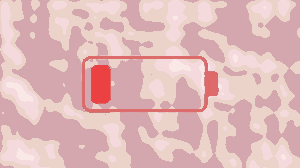
\includegraphics[width=0.5\linewidth,height=\textheight,keepaspectratio]{graphics/battery_i.png}

\subsection{Conclusion: Why Newton's Method
Wins}\label{conclusion-why-newtons-method-wins}

\begin{enumerate}
\def\labelenumi{\arabic{enumi}.}
\tightlist
\item
  \textbf{Quadratic Convergence}: Errors square each iteration
\item
  \textbf{Predictable Energy Cost}: O(n × log(precision))
\item
  \textbf{Scale Independence}: Input magnitude doesn't matter
\item
  \textbf{Hardware Friendly}: Simple arithmetic operations
\item
  \textbf{Memory Efficient}: Constant space complexity
\item
  \textbf{Universally Applicable}: Any nth root with same efficiency
\end{enumerate}

\begin{center}\rule{0.5\linewidth}{0.5pt}\end{center}

\begin{tcolorbox}[enhanced jigsaw, rightrule=.15mm, colbacktitle=quarto-callout-tip-color!10!white, titlerule=0mm, toptitle=1mm, colframe=quarto-callout-tip-color-frame, bottomtitle=1mm, coltitle=black, arc=.35mm, breakable, title=\textcolor{quarto-callout-tip-color}{\faLightbulb}\hspace{0.5em}{🌟 The Big Picture}, bottomrule=.15mm, toprule=.15mm, colback=white, left=2mm, opacityback=0, opacitybacktitle=0.6, leftrule=.75mm]

Newton's method represents a perfect balance of:

\begin{itemize}
\tightlist
\item
  {\textbf{Mathematical elegance}} ✨
\item
  {\textbf{Computational efficiency}} ⚡\\
\item
  {\textbf{Energy consciousness}} 🌱
\end{itemize}

\textbf{Result}: Sustainable, fast, and beautiful mathematics!

\end{tcolorbox}

\subsection{Questions \& Discussion}\label{questions-discussion}

\textbf{How might energy considerations influence algorithm choice in
your projects?}

\subsubsection{Try it yourself!}\label{try-it-yourself}

\begin{Shaded}
\begin{Highlighting}[]
\CommentTok{\# Experiment with different roots and values}
\NormalTok{result }\OperatorTok{=}\NormalTok{ newtons\_nth\_root(}\DecValTok{7}\NormalTok{, }\DecValTok{128}\NormalTok{, verbose}\OperatorTok{=}\VariableTok{True}\NormalTok{)}
\end{Highlighting}
\end{Shaded}

\subsection{Appendix: Complete
Implementation}\label{appendix-complete-implementation}

\begin{Shaded}
\begin{Highlighting}[]
\KeywordTok{def}\NormalTok{ newtons\_nth\_root\_complete(n: }\BuiltInTok{int}\NormalTok{, value: }\BuiltInTok{float}\NormalTok{, guess: }\BuiltInTok{float} \OperatorTok{=} \FloatTok{1.0}\NormalTok{, verbose: }\BuiltInTok{bool} \OperatorTok{=} \VariableTok{True}\NormalTok{) }\OperatorTok{{-}\textgreater{}} \BuiltInTok{tuple}\NormalTok{:}
    \CommentTok{"""}
\CommentTok{    Complete instrumented version with full energy analysis}
\CommentTok{    """}
    \ControlFlowTok{if}\NormalTok{ n }\OperatorTok{\textless{}=} \DecValTok{0}\NormalTok{:}
        \ControlFlowTok{raise} \PreprocessorTok{ValueError}\NormalTok{(}\StringTok{"n must be a positive integer"}\NormalTok{)}
    \ControlFlowTok{if}\NormalTok{ value }\OperatorTok{\textless{}} \DecValTok{0} \KeywordTok{and}\NormalTok{ n }\OperatorTok{\%} \DecValTok{2} \OperatorTok{==} \DecValTok{0}\NormalTok{:}
        \ControlFlowTok{raise} \PreprocessorTok{ValueError}\NormalTok{(}\StringTok{"Cannot find even root of negative number"}\NormalTok{)}
    
\NormalTok{    tolerance }\OperatorTok{=} \FloatTok{0.0001}
\NormalTok{    iterations }\OperatorTok{=} \DecValTok{0}
\NormalTok{    operations\_count }\OperatorTok{=} \DecValTok{0}
\NormalTok{    start\_time }\OperatorTok{=}\NormalTok{ time.time()}
    
    \ControlFlowTok{while} \BuiltInTok{abs}\NormalTok{(guess}\OperatorTok{**}\NormalTok{n }\OperatorTok{{-}}\NormalTok{ value) }\OperatorTok{\textgreater{}}\NormalTok{ tolerance:}
\NormalTok{        iterations }\OperatorTok{+=} \DecValTok{1}
        
        \ControlFlowTok{if}\NormalTok{ verbose:}
            \BuiltInTok{print}\NormalTok{(}\SpecialStringTok{f"Iteration }\SpecialCharTok{\{}\NormalTok{iterations}\SpecialCharTok{\}}\SpecialStringTok{: n = }\SpecialCharTok{\{}\NormalTok{n}\SpecialCharTok{\}}\SpecialStringTok{, value = }\SpecialCharTok{\{}\NormalTok{value}\SpecialCharTok{\}}\SpecialStringTok{, guess = }\SpecialCharTok{\{}\NormalTok{guess}\SpecialCharTok{\}}\SpecialStringTok{"}\NormalTok{)}
            \BuiltInTok{print}\NormalTok{(}\SpecialStringTok{f"   abs(guess\^{}n {-} value) = }\SpecialCharTok{\{}\BuiltInTok{abs}\NormalTok{(guess}\OperatorTok{**}\NormalTok{n }\OperatorTok{{-}}\NormalTok{ value)}\SpecialCharTok{\}}\SpecialStringTok{"}\NormalTok{)}
        
        \CommentTok{\# Detailed operation counting}
\NormalTok{        operations\_this\_iteration }\OperatorTok{=}\NormalTok{ (n}\OperatorTok{{-}}\DecValTok{1}\NormalTok{) }\OperatorTok{+}\NormalTok{ (n}\OperatorTok{{-}}\DecValTok{2}\NormalTok{) }\OperatorTok{+} \DecValTok{3} \OperatorTok{+} \DecValTok{2}
\NormalTok{        operations\_count }\OperatorTok{+=}\NormalTok{ operations\_this\_iteration}
        
\NormalTok{        guess\_new }\OperatorTok{=}\NormalTok{ guess }\OperatorTok{{-}}\NormalTok{ (guess}\OperatorTok{**}\NormalTok{n }\OperatorTok{{-}}\NormalTok{ value) }\OperatorTok{/}\NormalTok{ (n }\OperatorTok{*}\NormalTok{ guess}\OperatorTok{**}\NormalTok{(n}\OperatorTok{{-}}\DecValTok{1}\NormalTok{))}
        
        \ControlFlowTok{if}\NormalTok{ verbose:}
            \BuiltInTok{print}\NormalTok{(}\SpecialStringTok{f"   new\_guess = }\SpecialCharTok{\{}\NormalTok{guess\_new}\SpecialCharTok{\}}\SpecialStringTok{"}\NormalTok{)}
            \BuiltInTok{print}\NormalTok{(}\SpecialStringTok{f"   Operations this iteration: }\SpecialCharTok{\{}\NormalTok{operations\_this\_iteration}\SpecialCharTok{\}}\SpecialStringTok{"}\NormalTok{)}
        
\NormalTok{        guess }\OperatorTok{=}\NormalTok{ guess\_new}
    
\NormalTok{    computation\_time }\OperatorTok{=}\NormalTok{ time.time() }\OperatorTok{{-}}\NormalTok{ start\_time}
    
    \ControlFlowTok{if}\NormalTok{ verbose:}
        \BuiltInTok{print}\NormalTok{(}\SpecialStringTok{f"Convergence in }\SpecialCharTok{\{}\NormalTok{iterations}\SpecialCharTok{\}}\SpecialStringTok{ iterations"}\NormalTok{)}
        \BuiltInTok{print}\NormalTok{(}\SpecialStringTok{f"Total operations: }\SpecialCharTok{\{}\NormalTok{operations\_count}\SpecialCharTok{\}}\SpecialStringTok{"}\NormalTok{)}
        \BuiltInTok{print}\NormalTok{(}\SpecialStringTok{f"Computation time: }\SpecialCharTok{\{}\NormalTok{computation\_time}\SpecialCharTok{:.6f\}}\SpecialStringTok{ seconds"}\NormalTok{)}
    
    \ControlFlowTok{return}\NormalTok{ guess, iterations, computation\_time, operations\_count}
\end{Highlighting}
\end{Shaded}





\end{document}
